% !TEX TS-program = pdflatex
% !TEX encoding = UTF-8 Unicode

% This is a simple template for a LaTeX document using the "article" class.
% See "book", "report", "letter" for other types of document.

\documentclass[12pt]{article} % use larger type; default would be 10pt

\usepackage[utf8]{inputenc} % set input encoding (not needed with XeLaTeX)

%%% Examples of Article customizations
% These packages are optional, depending whether you want the features they provide.
% See the LaTeX Companion or other references for full information.

%%% PAGE DIMENSIONS
\usepackage{geometry} % to change the page dimensions
\geometry{a4paper} % or letterpaper (US) or a5paper or....
% \geometry{margin=2in} % for example, change the margins to 2 inches all round
% \geometry{landscape} % set up the page for landscape
%   read geometry.pdf for detailed page layout information

\usepackage{graphicx} % support the \includegraphics command and options
\graphicspath{{./doc_images/}}


\usepackage[section]{placeins}
\usepackage{tikz}
\usepackage{etoolbox} % for \ifnumcomp
\usepackage{listofitems} % for \readlist to create arrays

\tikzset{>=latex} % for LaTeX arrow head
\colorlet{myred}{red!80!black}
\colorlet{myblue}{blue!80!black}
\colorlet{mygreen}{green!60!black}
\colorlet{mydarkred}{myred!40!black}
\colorlet{mydarkblue}{myblue!40!black}
\colorlet{mydarkgreen}{mygreen!40!black}
\tikzstyle{node}=[very thick,circle,draw=myblue,minimum size=22,inner sep=0.5,outer sep=0.6]
\tikzstyle{connect}=[->,thick,mydarkblue,shorten >=1]
\tikzset{ % node styles, numbered for easy mapping with \nstyle
  node 1/.style={node,mydarkgreen,draw=mygreen,fill=mygreen!25},
  node 2/.style={node,mydarkblue,draw=myblue,fill=myblue!20},
  node 3/.style={node,mydarkred,draw=myred,fill=myred!20},
}
\def\nstyle{int(\lay<\Nnodlen?min(2,\lay):3)} % map layer number onto 1, 2, or 3


% \usepackage[parfill]{parskip} % Activate to begin paragraphs with an empty line rather than an indent

%%% PACKAGES
\usepackage{booktabs} % for much better looking tables
\usepackage{array} % for better arrays (eg matrices) in maths
\usepackage{paralist} % very flexible & customisable lists (eg. enumerate/itemize, etc.)
\usepackage{verbatim} % adds environment for commenting out blocks of text & for better verbatim
\usepackage{subfig} % make it possible to include more than one captioned figure/table in a single float
% These packages are all incorporated in the memoir class to one degree or another...

%%% HEADERS & FOOTERS
\usepackage{fancyhdr} % This should be set AFTER setting up the page geometry
\pagestyle{fancy} % options: empty , plain , fancy
\renewcommand{\headrulewidth}{0pt} % customise the layout...
\lhead{}\chead{}\rhead{}
\lfoot{}\cfoot{\thepage}\rfoot{}

%%% SECTION TITLE APPEARANCE
\usepackage{sectsty}
\allsectionsfont{\sffamily\mdseries\upshape} % (See the fntguide.pdf for font help)
% (This matches ConTeXt defaults)

%%% ToC (table of contents) APPEARANCE
\usepackage[nottoc,notlof,notlot]{tocbibind} % Put the bibliography in the ToC
\usepackage[titles,subfigure]{tocloft} % Alter the style of the Table of Contents
\renewcommand{\cftsecfont}{\rmfamily\mdseries\upshape}
\renewcommand{\cftsecpagefont}{\rmfamily\mdseries\upshape} % No bold!

%%% END Article customizations

%%% The "real" document content comes below...

\title{Facial Matching in Electronic Voting Systems}
\author{Gama Marius Catalin}
\date{} % Activate to display a given date or no date (if empty),
         % otherwise the current date is printed 

\begin{document}
\maketitle

\section{Introduction}
	Facial recognition is present in numerous systems and procedures in the modern day, and the fact that consumer products such as mobile phones have implemented it successfully is proof that something led by big organizations such as companies and governments could yield positive results and a decrease in frauds when implemented for an electronic voting system.\cite{a2}
	The current romanian voting system has a lot of flaws, however I believe that the biggest one is the fact that there are only a few central locations where people may go and cast their vote, and also a lot of bureaucracy is involved, taking a lot of time from the voters and the managing staff.
	Small kiosks and stations could be scattered around general points of interest (town halls, public parks - for government managed polls; main halls, cafeterias - for companies) and here the voting system might be present, where the user will go and scan their IDs, and a camera will take the live feed of the person casting the vote and compare it to the picture found on the ID card or in a central database, only getting the vote through if the software gives it the green light.


\section{Approach}

\subsection{Detecting faces}

	A big part of setting up a facial recognition system is detecting if there is actually a face in the current frame, and that can be quite easily done with a series of cascading feature maps \cite{a3}\cite{v2} that go over each part of the input image and check if the given section passes all the given checks. 



	This approach is very reliable and it can yield very accurate results as the subject doesn't need to go out of it's way to stand a specific way in order to match the processed section of the video feed, however the process is quite computationally expensive, and as such it lead to unoperabe loading times for each frame, thus it came to my attention that as a proof of concept it shouldn't be used, however in a real application it might be a good idea to implement such a thing.

	
	\begin{figure}[!htbp]
	
	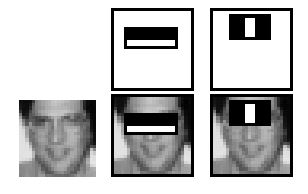
\includegraphics{cascading_features}
	\caption{Cascading feature maps used to detect faces}

	\end{figure}

	\FloatBarrier

\subsection{Comparing faces}

	Another key aspect of a facial matching system is that of actually managing to check if two given images share any kind of similarity, and as such an easy way of converting the given input to something that a computer can easily understand was needed, and as such the best approach was converting each image to a mathemathical equation \cite{v3}\cite{a1} that could be easily transformed and compared to another one of the same layout.




\section{Architecture}

	Given that the algorithm needed to take two images and process each one such that it could compare them in the end an architecture that took the greatest area of interest from each image and process it in a way that makes it able to be compared to the other one, such that a great approach that I found was using a convolutional siamese network \cite{a4} that works on two separete streams, one for each image, and in the end merges them to compare the two inputs.
	The network takes as input two images of shape 100x100x3 and processes them on three different sets of convolutional and max-pooling layers and then in the end another an additional convolutional and dense layer. This dense layer acts as the "equation" \cite{v3}\cite{a1}  that defines the given image. The comparison comes up as a L1 distance layer.


	\begin{figure}[!htb]
	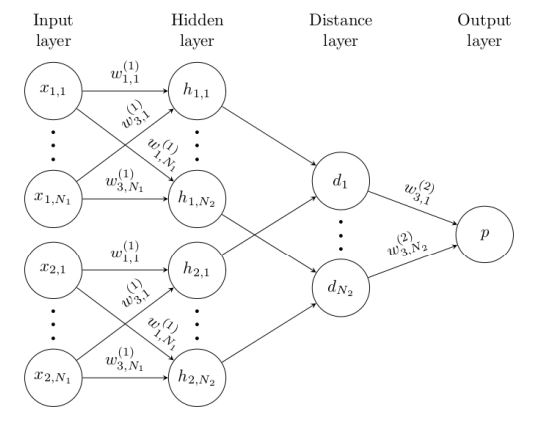
\includegraphics{siamese_network}
	\caption{Basic layout of the siamese neural network}
	\end{figure}


	\begin{figure}[!htb]
	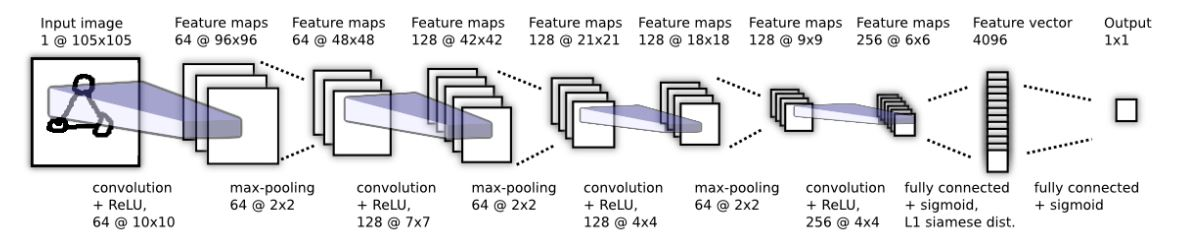
\includegraphics[scale=0.45]{siamese_network_layers}
	\caption{Layered view of the siamese network for one input, the siamese twin joins after the 4096 dense layer}
	\end{figure}




\section{Experimentation}

\subsection{Training}

	The network was trained using sets of 300 anchor, positive and negative images containing faces.
	Both the anchor and positive sets of images were recorded on the spot by taking pictures using the CV2 Python library through the webcam of the device, and the negative samples were part of the "Faces in The Wild" dataset.

	 The training procedure was run for 50 epochs, and each pair of images took my system ~14-17ms, definetely could be improved if the training was done on a GPU, and the accuracy of the network could have been even greater of more epochs or more samples were used.


\subsection{Testing}

	\subsubsection{Automated testing}

	A batch of 30\% of the used dataset was reserved for testing, and after two training iterations the results were almost 100\% for each test run that I did

	\subsubsection{Live testing}

	For live testing the siamese network was embeded into a live iteration of the application, where the user could validate the input taken from the device's webcam, and it was checked against a preset image that was used for validation (something similar to what a mobile phone has for FaceID).
	As expected, the failure rate of this iteration of the application was higher than that of the automated testing, resulting in ~70-80\% accuracy, however this number can be improved using a combination of more training runs or different threshold values for the validation of the image.


\section{Closing Statement}

	The siamese neural network \cite{a4} that I have used for this experiment needs a little bit more polish and an integration with a facial detection algorithm\cite{v2}\cite{a3} in order to be let out in the real world, however as a proof of concept for what can be done with relative ease for integrating a facial matcher into different applications it should be considered a successful experiment.


\bibliographystyle{plain}
\bibliography{bib_references.bib}

\end{document}
